\chapter{Parallele Rechnerarchitekturen}

\section{Supercomputer}
Ein Supercomputer ist typischerweise sehr schnell - klar. Aber für die Wissenschaftler, welche ihn einsetzen, ist er immer noch viel zu langsam. Es werden zwei Arten von Supercomputer unterschieden:

\begin{description}
	\item[Cluster of Server (Kernel level cluster): ] Hochverfügbare Rechner, welche wissen was die anderen Rechner um sie herum gerade tun. Sind über hochverfügbare Netzwerke untereinander verbunden.
	\item[Cluster of Computing Nodes (grid):] Verteilte Rechnernodes, z.B. SETI@home. Die einzelnen Nodes wissen nicht, was die anderen tun und werden von einer zentralen Stelle aus gesteuert.
\end{description}

\subsection{Einsatzgebiete Supercomputer}
\begin{enumerate}
	\item Wettervorhersagen
	\item Fluiddynamische Berechnungen
	\item DNA Entschlüsselung
	\item ...
\end{enumerate}
Die Stärke von Supercomputern ist das Lösen von parallel lösbaren Problemen. Daher funktionieren Aufgaben wie z.B. eine Gleichung lösen auf einem Supercomputer sehr schnell, andere Aufgaben wie das Erstellen eines Index über eine Datenbank, gleich schnell wie auf einem einfachen PC.

\subsection{Infiniband}
Wird in Supercomputer verwendet zur Verbindung der einzelnen Nodes untereinander. Extrem schnell (bis 60Gbit/s). Gibt nur wenige Hersteller, daher sehr teuer.

\section{Processor-Level Parallelism}

\subsection{SMP - Symetric Multiprocessing}
Eine SMP Architektur besteht aus mehreren physischen Prozessoren. Diese physischen Prozessoren müssen alle dieselben Funktionen ausführen können. Das bedeutet, dass nun die laufenden Prozesse frei auf die Prozessoren verteilt werden können.
Das spezielle an symmetrischen Multiprozessoren ist, dass der Speicher und die I/O Geräte über alle Prozessoren hinweg geteilt wird, wie in Abbildung \ref{fig:mc_simple_chip} dargestellt ist. Sie sind über einen Bus zusammengeschaltet (Bottleneck), oder direkt z.B. via QPI (Intel QuickPath Interconnect). 

\subsection{CMP - Chip Level Multiprocessing}
Danach begann man, die einzelnen Prozessoren in einem einzelnen Chip zusammenzufassen, was in einer verdoppelten Performance pro Prozessorchip resultiert. Eine solche Architektur ist in Abbildung \ref{fig:mc_shared_cache_chip} zu sehen. 

\begin{figure}
	\centering
	\begin{subfigure}[b]{0.15\textwidth}
		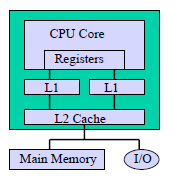
\includegraphics[width=\textwidth]{fig/mc_one}
		\caption{Konventioneller Mikroprozessor}
		\label{fig:mc_conventional}
	\end{subfigure}
	~
	\begin{subfigure}[b]{0.27\textwidth}
		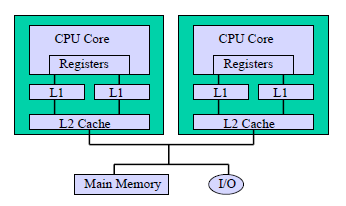
\includegraphics[width=\textwidth]{fig/mc_simple_chip}
		\caption{SMP-Architektur}
		\label{fig:mc_simple_chip}
	\end{subfigure}
	~
	\begin{subfigure}[b]{0.25\textwidth}
		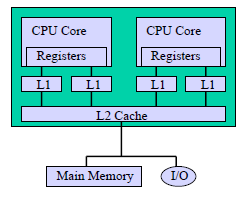
\includegraphics[width=\textwidth]{fig/mc_shared_cache}
		\caption{CMP-Architektur}
		\label{fig:mc_shared_cache_chip}
	\end{subfigure}
	~
	\begin{subfigure}[b]{0.25\textwidth}
		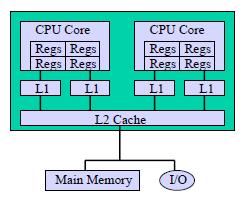
\includegraphics[width=\textwidth]{fig/mc_shared_cache_mt}
		\caption{CMT-Architektur}
		\label{fig:mc_shared_cache:mt}
	\end{subfigure}
	\caption{Verschiedene Prozessor Architekturen}
	\label{fig:cache_strukturen}
\end{figure}

\section{Instruction-Level Parallelism}

\subsection{Pipelines}
Instruktionen aus dem Memory zu holen ist extrem langsam. Um dieses Problem zu beheben, hatten Prozessoren schon früh die Möglichkeit, Instruktionen frühzeitig aus dem Memory zu holen, sodass sie bereitstanden wenn sie gebraucht wurden.
Man teilte daher die Instruktion in 2 Teile - Fetching und Execution. Das Konzept einer Pipeline geht hier noch weiter und unterteilt die Instruktion in noch mehr Teile, die alle von einem speziellen Stück Hardware ausgeführt werden - und dies erst noch parallel.

Die Abbildung \ref{fig:pipeline} zeigt eine solche Pipeline mit 5 Schritten. Zuerst wird die Instruktion geholt, danach wird entschieden was für eine es ist und was für Operanden gebraucht werden. Anschliessend werden diese Operanden geholt und die eigentliche Instruktion ausgeführt. Abschliessend wird das Resultat gespeichert oder weiterverarbeitet.
\begin{figure}[h!]
	\centering
	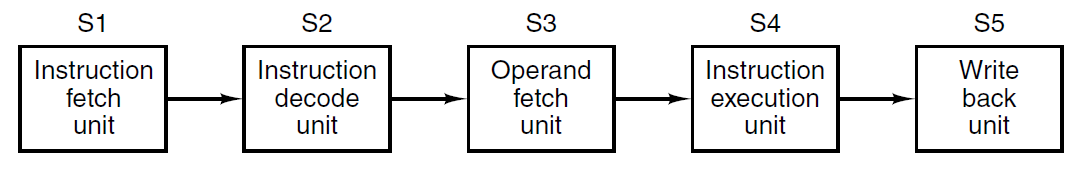
\includegraphics[width=0.7\linewidth]{fig/pipeline}
	\caption{Pipeline}
	\label{fig:pipeline}
\end{figure}

\subsection{Superskalare Architektur}
Ein zweiter, unabhängiger Ansatz ist es, dass man nebst einer Pipeline auch noch die Instruktionsausführung parallelisiert, da eine Instruktionsausführung einiges länger dauert als z.B das Verarbeiten des Resultats. Dabei wird die Tatsache ausgenutzt, dass eine Instruktion auf einem Prozessor z.B. nur die ALU, die nächste Instruktion nur den Bitshifter braucht. Daher kann man diese Instruktionen parallelisiert ausführen, d.h. gleichzeitig eine Multiplikation und ein Bitshift, auf getrennten Bereichen auf der CPU. Abbildung \ref{fig:superskalar} zeigt ein Design einer solchen Superskalaren Architektur.
\begin{figure}
\centering
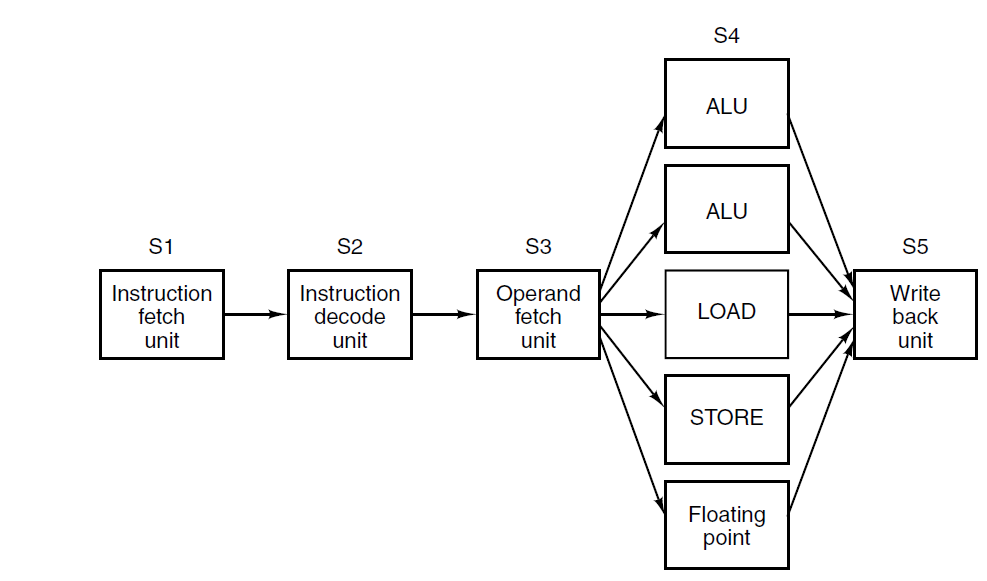
\includegraphics[width=0.7\linewidth]{fig/superskalar}
\caption{Superskalare Architektur}
\label{fig:superskalar}
\end{figure}

\section{SMT - Simultanous Multithreading}
Superskalare Architekturen tönen super gut, haben allerdings auch ihre Limitierungen. Wenn zwei Instruktionen voneinander abhängen, können sie nicht gleichzeitig auf die Recheneinheiten gelegt werden, was bedeutet, dass in der Praxis nie alle Recheneinheiten einer CPU gleichzeitig ausgelastet werden können, da die Applikation dies so nicht zulässt.

In einer Umgebung mit vielen Threads (auf dem Computer, auf dem dieser Text geschrieben wurde, laufen im Moment über 1'000 Threads gleichzeitig), können nun mit einer SMT Architektur in jedem Prozesszyklus mehrere Threads gleichzeitig auf demselben Prozessorkern rechnen, da die Instruktionen auf mehrere Einheiten verteilt werden (die eine braucht die ALU, die andere die FPU, ...). Da genügend Threads mit Instruktionen zur Auswahl stehen, kann der Prozessor auch einfach auswählen, welche Instruktionen als nächstes ausgeführt werden. So können alle Funktionseinheiten der CPU optimal ausgelastet werden.

Um eine solche Architektur in Hardware zu implementieren, benötigt es einfach mehr Register für die einzelnen Threads, sowie eine zusätzliche Kontrolleinheit in der Pipeline um die Threads auf dem Prozessor zu verteilen.

\subsection{CMT - Chip Level Multithreading}
Wenn man nun mehrere Prozessoren auf demselben Chip hat und zusätzlich noch Multithreading anwendet, hat man eine Chip Level Multithreading Architektur (CMP + SMT = CMT). Wird heute angewendet.

\section{Klassifikation nach Flynn}
\begin{figure}
\centering
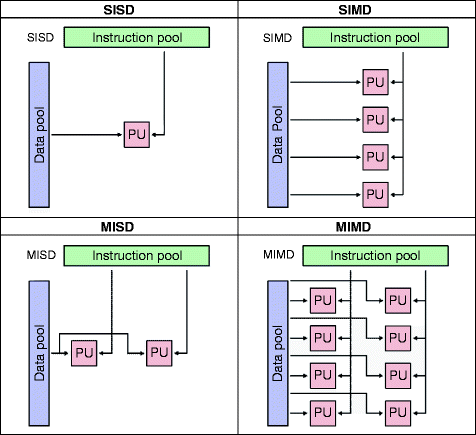
\includegraphics[width=0.5\linewidth]{fig/flynn}
\caption{}
\label{fig:flynn}
\end{figure}
\begin{description}
	\item[Single Instruction Single Data:] Ein klassischer Von-Neumann-Rechner
	\item[Single Instruction Multiple Data:] Ein Vektorrechner, VLIW-Rechner
	\item[Multiple Instruction Single Data:]	Sehr selten, eingesetzt für Machine Learning oder fehlerresistente Berechnung
	\item[Multiple Instruction Multiple Data:] Parallellrechner, moderne symmetrische Multiprozessoren
\end{description}

\newpage

\section{Speicherorganisation in SMP Rechnern}

\subsection{Shared Memory Architektur}
Wir haben mehrere Prozessoren, die miteinander ein Rechner bilden, d.h. ein MIMD Rechner (SMP). Dabei sollen alle das Memory teilen, in einem grossen, global adressierten Speicher. Dies bietet den Vorteil einer hohen Kommunikationsleistung, kleiner Latenz, kleiner Hardwareaufwand und einfacher Programmierung.

\subsection{Private Memory}
Hier hat jeder Knoten seinen eigenen Speicher. Dabei wird nicht über einen gemeinsamen Adressraum kommuniziert, sondern via Nachrichten. Das bedeutet höhere Administrationskosten, ein langsameres Netzwerk als via einen Bus, welches dafür sehr einfach erweiterbar ist.
Prozessoren haben sonst nur Zugriff auf ihren eigenen Speicher.

\subsubsection{UMA - Uniform Memory Access}
Hier ist die Speicherzugriffszeit gleich (uniform) für alle Adressen. Dabei wird üblicherweise ein gemeinsamer, zentraler Speicher eingesetzt.
\begin{figure}[h!]
\centering
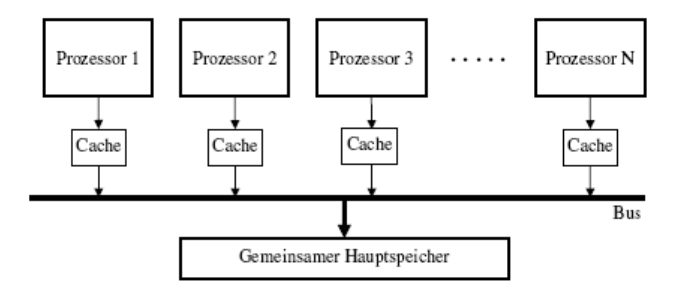
\includegraphics[width=0.5\linewidth]{fig/uma}
\caption{UMA Architektur}
\label{fig:uma}
\end{figure}

\subsubsection{NUMA - Non-Uniform Memory Access}
Die Zugriffszeit ist nicht für alle Speicherbereiche gleich, weil der Speicher verteilt ist.
\begin{figure}[h!]
\centering
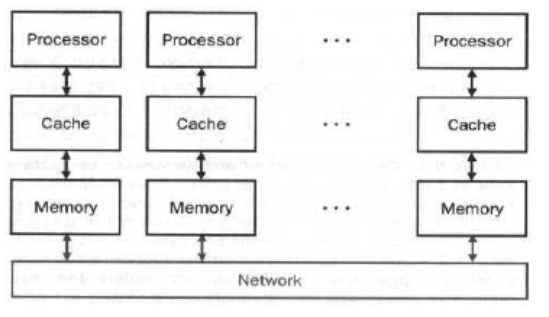
\includegraphics[width=0.5\linewidth]{fig/numa}
\caption{NUMA Architektur}
\label{fig:numa}
\end{figure}

\section{Mirrored Memory}
Dabei wird einfach RAM von einigen RM Modulen auf andere dupliziert. Soll die Ausfallsicherheit erhöhen im Falle eines Fehlers des RAM Moduls. Bringt in der Praxis nicht wirklich viel.

\section{Amdahls Gesetz}
Besagt, dass Programme nur bis zu einem gewissen Punkt parallelisierbar sind, denn irgendwo gibt es Punkte, welche nicht parallelisierbar sind. Sagen wir, 20\% eines Programms ist nicht parallelisierbar. Beim Hinzufügen von Prozessoren sinkt die Ausführungszeit des Programms immer mehr, unterschreitet jedoch niemals die 20\%, welche nicht parallelisierbar sind. 
Für die Berechnung der relativen Rechenzeit gilt die Formel \ref{eq:amdahl}.
\begin{equation}\label{eq:amdahl}
Relative\ Rechenzeit\ T = a + \frac{1-a}{n}
\end{equation}
$ a $ ist dabei der nicht parallelisierbare Anteil. Ein Programm auf einem Prozessor ($ n $) benötigt daher eine Rechenzeit von 1. Mit 2 Prozessoren sind es nur noch 0.6, mit 10 0.28 und mit 100 0.202. Es ist klar, dass der Wert daher gegen 0.2 konvergiert.
Abbildung \ref{fig:amdahl} soll dies verdeutlichen.
\begin{figure}[h!]
\centering
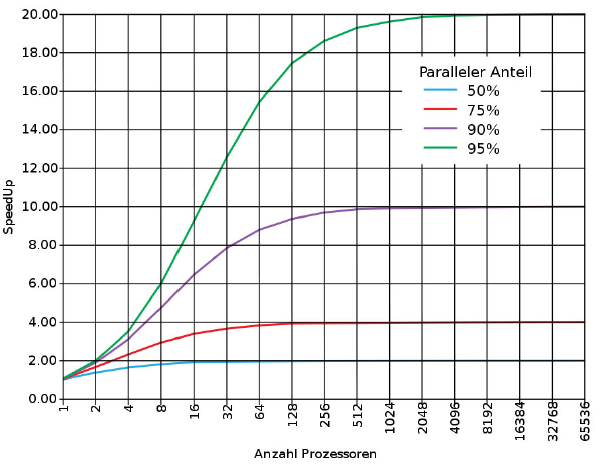
\includegraphics[width=0.5\linewidth]{fig/amdahl}
\caption{Amdahls Gesetz}
\label{fig:amdahl}
\end{figure}
Die relative Leistung eines Programms ist definiert als die Umkehrung von der relativen Rechenzeit, wie in Formel \ref{eq:amdahl_leistung} abgebildet.

\begin{equation}\label{eq:amdahl_leistung}
	Leistung\ P = \frac{1}{Relative\ Rechenzeit\ T }
\end{equation}

\section{Cachekohärenz}

\subsection{Write Through vs. Write Back}
Beim Write Through Cache wird der Hauptspeicher beim Verändern des Caches ebenfalls verändert. Beim Write Back Cache wird der Hauptspeicher nicht sofort verändert.
 
\subsection{Probleme mit Caches}
Das Problem bei beiden Verfahren ist, dass andere Prozessoren von der Variable alte, nicht mehr gültige Werte im Cache haben können.

\subsection{Cachekohärenzprotokolle}

\subsubsection{Snoopy}
Da ja alle Zugriffe über einen gemeinsamen Bus oder Switch laufen, können alle Prozessoren den Bus beobachten und erkennen, welche Blöcke wo von wem gespeichert sind. Dies skaliert allerdings nicht sonderlich gut (mehr als 64 Prozessoren liegen da nicht drin), da der Bus zu wenig Bandbreite besitzt.

\begin{figure}[h!]
\centering
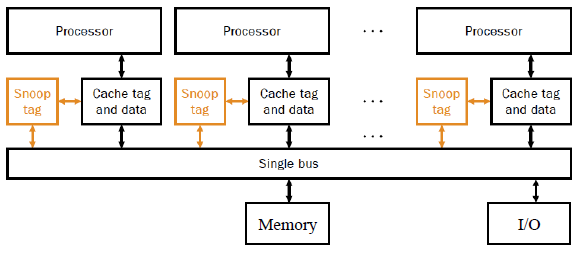
\includegraphics[width=0.5\linewidth]{fig/snoopy}
\caption{Snoopy Protokoll}
\label{fig:snoopy}
\end{figure}

Der Cache kann dargestellt werden als eine einfache Liste von Speicherblöcken, welche nun zusätzlich noch ein Status Flag haben, welches verschiedene Werte annehmen kann. Wenn z.B. nun irgendwo auf dem Bus ein Prozessor den Wert einer Variable ändert die im Cache eines anderen Prozessors bereits vorhanden ist, merkt das der andere Cache und setzt seinen Cache eintrag auf 'invalid'.

\subsubsection{Directory}
Eine zentrale Liste mit allen Cache Blöcken darin. Zusätzlich wird notiert, welcher Prozessor welche Cache Blöcke besitzt, zusammen mit dem aktuellen Zustand (z.B. dass er überall up-to-date ist, oder dass er nirgends drin ist usw.).

Wenn wir nun eine Architektur haben, bei denen mehrere Prozessoren involviert sind und diese je ein eigenes Memory haben, hat jeder Prozessor dazu noch sein eigenes Cache Directory, in dem Informationen über die Blöcke in diesem Speicher notiert sind.

\begin{figure}[h!]
\centering
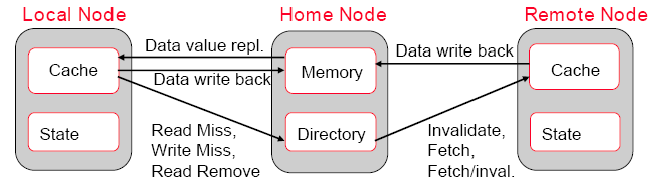
\includegraphics[width=0.7\linewidth]{fig/directory_protocol}
\caption{Directory Protokoll}
\label{fig:directory_protocol}
\end{figure}

Abbildung \ref{fig:directory_protocol} zeigt die Vorgehensweise (Node = Prozessor). Der Local Node möchte eine Operation auf einem Speicherbereich durchführen, welcher nicht in seinem lokalen Memory liegt. Er fragt den Home Node des Speicherbereichs, was denn der aktuelle Wert ist. Nach der Operation schreibt er die Daten zurück in den Hauptspeicher, welcher alle Kopien vom Cache benachrichtigt.

\subsection{Gemeinsamer Cache}
Grösserer Hardwareaufwand und Speicherzugriffe sind sequentialisiert -  d.h. langsamer.

\subsection{Unterteilung der Daten}
Bei Daten, die von mehreren Prozessoren verwendet werden, gibt es jeweils nur eine Kopie. Die Unterteilung übernimmt die Software selbst, indem es das Programm in Abschnitte unterteilt. Nach jedem Abschnitt werden alle Caches in den Speicher geschrieben (Cache flush). Wenn die Abschnitte zu klein sind, gibt es zu viele Cache Flushes, wenn sie zu gross sind können die Programme nicht effizient parallelisiert werden. Dieser Ansatz ist nicht sonderlich effizient, da es von konservativen Annahmen ausgeht.
 
\section{Verbindungsnetzwerke}
Wenn man mehrere Prozessoren und Speicher hat möchte man diese möglichst effizient miteinander verbinden. Man möchte diesen Verbindungen eine möglichst hohe Leistung haben. Das heisst, dass man viele Leitungen benötigt. Gleichzeitig möchte man niedrige Kosten, was heisst dass man nur wenig Leitungen einsetzen darf. Die Verbindungsnetzwerke werden mit folgenden Kennwerten klassifiziert:
\begin{description}
	\item[Inzident:] Wenn Kante und Knoten verbunden sind, sind sie inzident.
	\item[Durchmesser:] Max. Entfernung zwischen zwei Knoten in Hops (Mass für max. Transferzeit).
	\item[Bisektionsweite:] Möchte man ein Netzwerk halbieren ist die Bisektionsweite die Anzahl Kanten die man durchtrennen muss. Je niedriger die Bisektionsweite desto schlechter der Datenaustausch.
	\item[Symmetrie:] Alle Knoten/Kanten verhalten sich gleich. Vereinfacht Programmierung, Routing usw.
	\item[Skalierbarkeit:] Ein Verbindungsnetzwerk ist skalierbar, wenn einer Erweiterung des Netzwerks keine Beschränkungen entgegen stehen.
	\item[Konnektivität:] Min. Anzahl Kanten die durchtrennt werden müssen damit Netz nicht mehr funktioniert. Je höher die Konnektivität desto ausfallsicherer das Netz.
\end{description}

\subsection{Lineares Feld}
Unendlich skalierbar (hardwaretechnisch gesehen), offensichtliche Limitierungen bei der Bandbreite und Latenz.

\begin{figure}[h!]
	\centering
	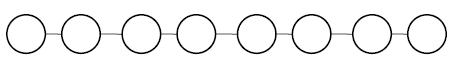
\includegraphics[width=0.7\linewidth]{fig/lineares_feld}
	\caption{Lineares Feld}
	\label{fig:lineares_feld}
\end{figure}

\subsection{Ring}
Ebenfalls unbeschränkt skalierbar. Wenn in beide Richtungen traversierbar, ist die maximale Latenz die Hälfte aller Knoten.

\begin{figure}[h!]
	\centering
	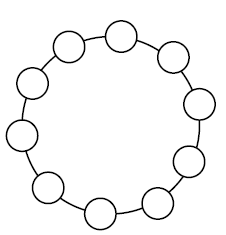
\includegraphics[width=0.2\linewidth]{fig/ring}
	\caption{Ring}
	\label{fig:ring}
\end{figure}

\subsection{Stern}
Alle Kommunikation läuft via das Zentrum des Sterns, daher nicht skalierbar. Dafür sehr grosse Bandbreite und niedrige Latenz.

 \begin{figure}[h!]
\centering
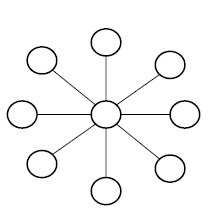
\includegraphics[width=0.2\linewidth]{fig/stern}
\caption{Stern}
\label{fig:stern}
\end{figure}

\subsection{Baum}
Der Baum ist sehr gut skalierbar und bietet eine ausgewogene Latenz. Dafür kann die Bandbreite eingeschränkt sein.

\begin{figure}[h!]
	\centering
	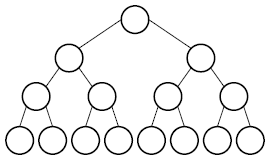
\includegraphics[width=0.2\linewidth]{fig/baum}
	\caption{Baum}
	\label{fig:baum}
\end{figure}

\subsection{Hypercube}
Mässige Skalierbarkeit. Bietet eine gute Bandbreite, da viele Kanten vorhanden sind. Latenz steigt logarithmisch mit Anzahl der Knoten. Abbildung \ref{fig:hypercube_impl} zeigt eine Implementierung einer Hypercube Struktur in Prozessoren.

\begin{figure}[h!]
\centering
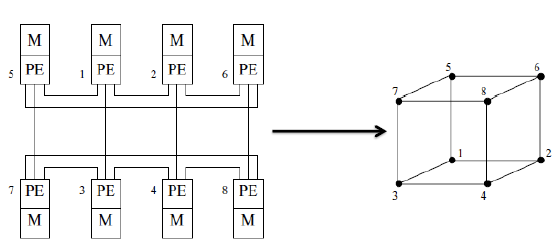
\includegraphics[width=0.5\linewidth]{fig/hypercube_impl}
\caption{Hypercube Implementation}
\label{fig:hypercube_impl}
\end{figure}

\subsection{Koppelnetze}

\subsubsection{Crossbar Switch}
Heute das beste und meist verwendetste Layout. Es ist nicht blockierend und verbindet eine Menge von Geräten untereinander. Wenn 2 Geräte (oder ein Prozessor und ein Speichermodul) Daten austauschen, kann das einen anderen Prozessor nicht beeinflussen, da zu jedem Zeitpunkt immer eine Route zum Speichergerät zur Verfügung steht. Abbildung \ref{fig:crossbar_switch} zeigt einen solchen Crossbar Switch. Der gezeigte Crossbar Switch verbindet zur Zeit gleichzeitig 3 CPUs und Memories, verbunden durch die geschlossenen Kreuzungspunkte. Das bedeutet auch, dass ein Crossbar Switch UMA ist, d.h. alle Speicherstellen können mit derselben Latenz angesprochen werden.
\begin{figure}[h!]
\centering
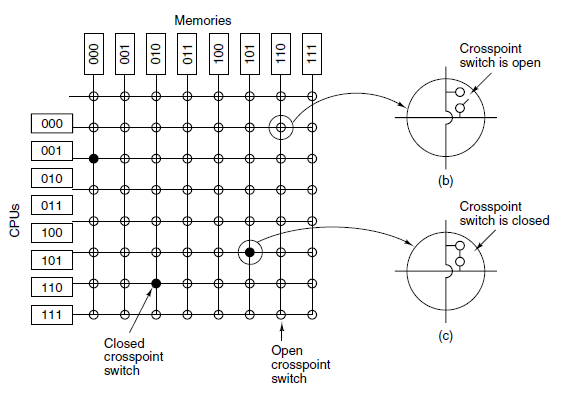
\includegraphics[width=0.5\linewidth]{fig/crossbar_switch}
\caption{Ein 8x8 Crossbar Switch}
\label{fig:crossbar_switch}
\end{figure}

Der Nachteil bei Crossbar Switches ist die mangelnde Skalierbarkeit, denn die Anzahl an Knoten wächst im Quadrat mit der Anzahl der zu verbindenden Elemente. Wenn z.B. 1'000 CPUs mit 1'000 Memory Modulen verbunden werden sollen, würde es eine Million Kreuzungspunkte benötigen, was nicht gerade effizient wäre.

\subsubsection{Omega Netzwerk}
Stellen wir uns einen simplen 2x2 Switch vor, mit zwei Eingängen und zwei Ausgängen, siehe Abbildung \ref{fig:omegaswitch}. Unser kleiner Switch erhält eine (hier vereinfachte) Nachricht bestehend aus 4 Elementen. Das \texttt{Module}-Feld, gibt an, welches Memory-Modul benützt werden soll. Das \texttt{Address}-Feld sagt, an welche Adresse sich die Nachricht richtet. Das \texttt{Opcode}-Feld bestimmt, ob es eine Lese- oder eine Schreiboperation ist und schlussendlich das \texttt{Value}-Feld welche Daten denn geschrieben werden sollen, wenn es eine Schreiboperation ist.
\begin{figure}[h]
	\centering
	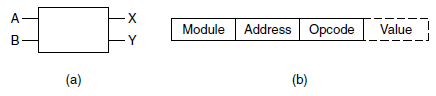
\includegraphics[width=0.7\linewidth]{fig/omega_switch}
	\caption{(a) Ein 2x2 Switch. (b) Das Nachrichten Format}
	\label{fig:omegaswitch}
	\end{figure}

Ein solch kleines Netzwerk bringt uns noch nicht weit, weswegen wir nun 8 Prozessoren und 8 Speicher nehmen. Wir können nun mittels 12 solcher einfacher Switches alle 8 CPUs mit allen 8 Memories verbinden, wie in Abbildung \ref{fig:omega_gross} gezeigt.
\begin{figure}[h]
	\centering
	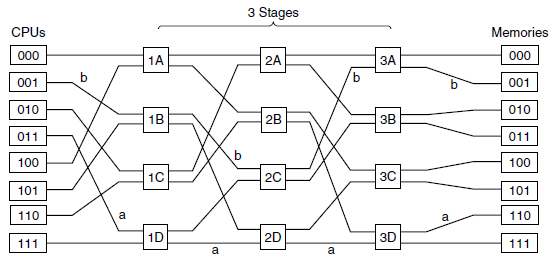
\includegraphics[width=0.7\linewidth]{fig/omega_gross}
	\caption{Ein Omega Netzwerk mit 8 CPUs und 8 Speicher}
	\label{fig:omega_gross}
	\end{figure}
Dieses gezeigte Netzwerk wird \textbf{Omega Netzwerk} genannt. Es verbindet via 3 Stufen die 8 CPUs mit den Memories. Wir können auch sagen, für $ n $ CPUs und Memories benötigen wir $ log_{2}\ (n) $ Stufen und total $ \frac{n}{2}\ log_{2}\ (n) $ Switches, was einiges besser als das Crossbar Netzwerk ist, welches ja $ n^{2} $ Kreuzungspunkte benötigt. Im Beispiel mit den 8 Prozessoren werden daher nicht 64 Kreuzungspunkte wie beim Crossbar Switch benötigt, sondern nur 12 Switches. Der Nachteil vom Omega Netzwerk ist, dass es blockierend ist. Wenn nun z.B. die 2 Prozessoren 000 und 100 gleichzeitig auf eine Memory Stelle zugreifen möchten, muss ein Prozessor warten, da sie via denselben Switch zugreifen müssen.

\section{Applikationsskalierung}
Gemeinsame Zustände in die Datenbank verlegen (oder auslagern). Skalierbare Algorithmen verwenden. Fein granulares Locking verwenden, Worker Thread Pools verwenden. Natürlich auch immer Skalierungs-Tests durchführen, sowie die Applikation im Betrieb beobachten und Orte identifizieren, wo gewartet werden muss, sei dies wegen locks oder falschen Algorithmen, etc.